\chapter{Evaluation}	\label{ch:evaluation}
The evaluation is divided into four sections, first a section describing the web application developed, section~\ref{sec:web-application}, followed by one section for each framework used to develop the mobile application, sections~\ref{sec:native-android} and \ref{sec:phonegap}. Last in this chapter, is a section presenting the development effort of each mobile application, section~\ref{sec:development-effort}.

\section{Web Application}\label{sec:web-application}
To simplify the process of making the web application compatible with web browsers as well as the mobile application, the architecture follows the Adapter pattern \cite[p.~317]{martin2003}. The structure of the web application can be seen in figure \ref{fig:webuml}. Items within the red dotted box belong to the structure when the Android framework was used for developing the mobile application. Items within the blue dotted box belong to the structure when the PhoneGap framework was used for developing the mobile application.

\begin{figure}[h!]
	\centering
    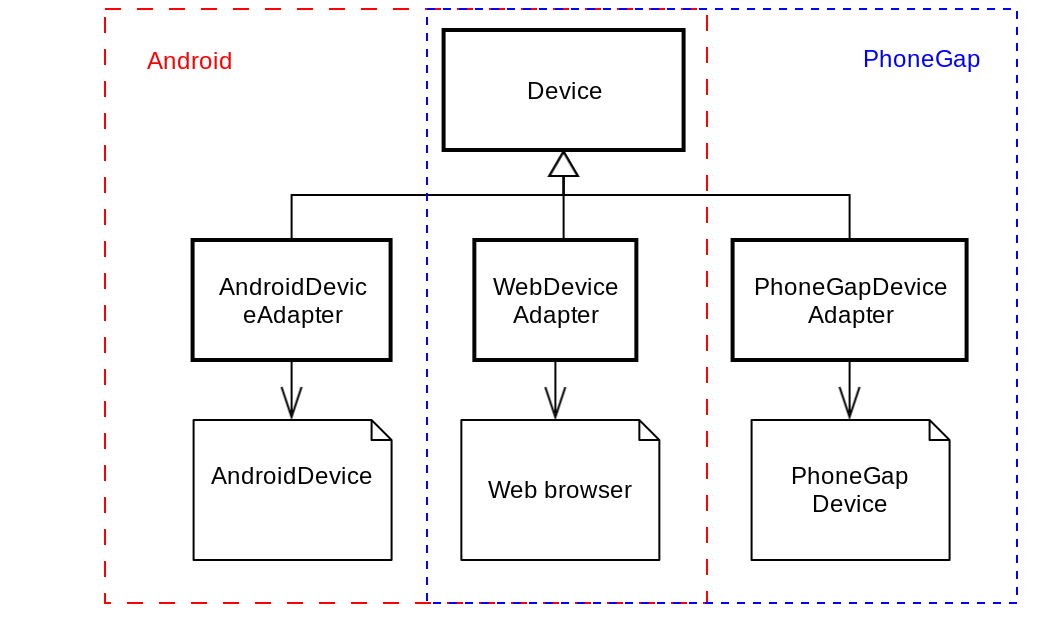
\includegraphics[width=90mm,natwidth=600,natheight=450]{./img/webuml.png}
    \caption{Structure of the web application}
	\label{fig:webuml}
\end{figure}

\section{Native android} \label{sec:native-android}
The mobile application developed in the Android framework can be found on Github at \url{https://github.com/buren-trialbee/pollux}. An overview of the application structure and functionality follows in section~\ref{subsec:mobile-application-structure-native}. After this, in section~\ref{subsec:function-flow-native}, a practical example is used to describe the flow of function calls when a native function is requested by the web application layer.

\subsection{Mobile Application structure} \label{subsec:mobile-application-structure-native}
The UI of the Android application consist of a single WebView \ref{subsubsec:webview} (used to load the web application). A UML-diagram representing the logic of the Android application can be seen in figure ~\ref{fig:nativeuml}. The contained classes are summarized below, with a short explanation followed by code examples.

\begin{figure}
	\centering
    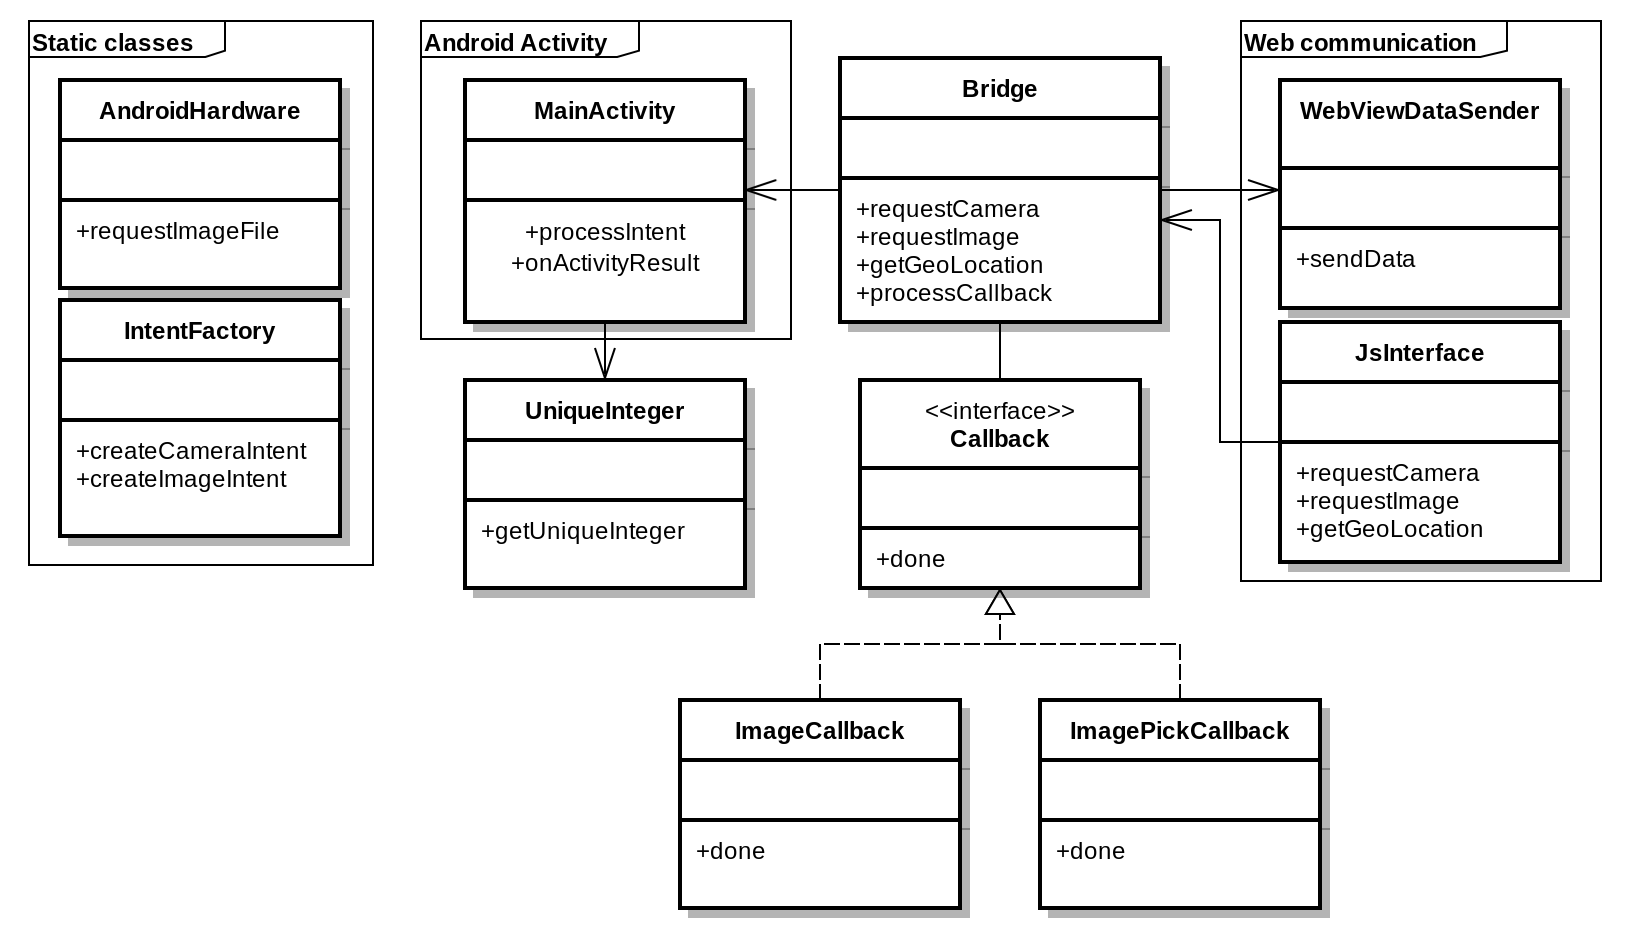
\includegraphics[width=150mm,natwidth=1000,natheight=750]{./img/polluxuml.png}
    \caption{Structure of the android application}
    \label{fig:nativeuml}
\end{figure}

\subsubsection{MainActivity} 
MainActivity is the main activity~\ref{subsubsec:activity} of the Android application. It contains logic for handling the application's activity lifecycle, and is in charge of starting any activities needed to provide the Web Application with data from native functions, such as the device camera. Activities are started by a call to the processIntent function. It takes an Intent \ref{subsubsec:intent} and a Callback (see section below) as arguments. The callback is provided a unique id, and is stored in a map. The Intent is started with the use of the startActivityForResult function provided by the Android SDK \ref{subsec:android-application-framework}, and is assigned a request id equal to the id of the Callback. 
\\\\
	
\emph{Ex. Starting an Activity for result}
\begin{lstlisting}
// Request a unique integer to use as id
int requestCode = uniqueInteger.getUniqueInteger();

// Store the Callback in a map with the unique integer as key	
callbacks.put(requestCode, callback);
   
// Start the Activity defined in the Intent, 
// assigning the unique integer as request code
startActivityForResult(intent, requestCode);
\end{lstlisting}
	
\subsubsection{IntentFactory} 
IntenFactory provides Intents \ref{subsubsec:intent} for native functions such as capturing an image or picking an image from the gallery.
	\\\\
	\emph{Ex. getting Intent from IntentFactory}
	
	\begin{lstlisting}
// In Bridge:
Intent imageIntent = IntentFactory.createCameraIntent(context);
		
// In IntentFactory:
public static Intent createCameraIntent(Context context) {
	// Create the intent for capturing an image
	Intent takePictureIntent = 
		new Intent(MediaStore.ACTION_IMAGE_CAPTURE);
	
	// Ensure that there's a camera activity to handle the intent
	if (takePictureIntent
		.resolveActivity(context.getPackageManager()) != null) {
		// Create the File where the photo should go
		File photoFile = AndroidHardware.requestImageFile();
		takePictureIntent.putExtra(MediaStore.EXTRA_OUTPUT,
		Uri.fromFile(photoFile));
	}
	return takePictureIntent;
}
\end{lstlisting}
	
\subsubsection{AndroidHardware}
AndroidHardware contains static methods, performing a single well-defined hardware related task. This design is chosen to make the application logic independent of the code in AndroidHardware. The code example below shows the function called to request a file for storing an image.
	\\\\
	\emph{Code example extracted from AndroidHardware:}
\begin{lstlisting}
public static File requestImageFile() {
 String fileName = "tempPhoto";
 File storageDir = 
   Environment.getExternalStoragePublicDirectory(
     Environment.DIRECTORY_PICTURES
     );
 File photoFile = null;
 try {
   photoFile = File.createTempFile(fileName, ".jpg", storageDir);
 } catch (IOException e) {
   e.printStackTrace();
 }
 return photoFile;
}
\end{lstlisting}
	
\subsubsection{Bridge} 
Bridge serves as a bridge between the mobile and web application layer. When the web application requests data from a native function, Bridge receives the request from JsInterface~\ref{subsubsec:jsinterface}, creates the corresponding Intent and Callback, and forwards them to MainActivity, see Ex. 1 below. Bridge also receives the result from the native function call, which it forwards to WebViewDataSender, see Ex. 2 below.
\\\\
\emph{Ex. 1 Processing a request for an image from the gallery}
\begin{lstlisting}
// Create a new intent
Intent imageIntent = IntentFactory.createImageIntent(context);

// Create callback for the intent
Callback imagePickCallback = new ImagePickCallback(this, context, callback);

// Send intent to mainActivity for processing
mActivity.processIntent(imageIntent, imagePickCallback);
\end{lstlisting}

\emph{Ex. 2 Forwarding data returned from native function}
\begin{lstlisting}
public void processCallback(String callback, String argument) {
        webViewDataSender.sendData(callback, argument);
}
\end{lstlisting}
	
\subsubsection{WebViewDataSender}
WebViewDataSender is in charge of all communication with the WebView and it's encapsulated web application. Upon application start, it loads the web application and injects the JavaScriptInterface. The class also contains logic for executing JavaScript functions in the web application, used to return results from native function calls.
\\\\
\emph{Ex. sendData - used by bridge to send back results to the web application}
\begin{lstlisting}
public void sendData(final String javascriptFunction, final String arg) {
        Log.d(TAG, "sendData");
        webView.post(new Runnable() {
            	@Override
            	public void run() {
        		webView.loadUrl("javascript:" + javascriptFunction + "('" + arg + "')");
    		}
	});
}
\end{lstlisting}
	
\subsubsection{JsInterface} \label{subsubsec:jsinterface}
JsInterface is exposed to the web application as a JavaScriptInterface and acts as a receiver for function calls from the web application. If the web application requires data from a native function, the JavaScript in the web application can call upon the proper method in JsInterface, which in turn forwards the requests to Bridge.
\\\\
\emph{Ex. Two java functions exposed to the web application by JsInterface}
\begin{lstlisting}
    //Request an image from the device camera
    @JavascriptInterface
    public void requestCamera(String callback) {
        Log.d(TAG, "requestImage");
        bridge.requestCamera(callback);
    }

    // Request an image from the device storage
    @JavascriptInterface
    public void requestImage(String callback) {
        Log.d(TAG, "requestImage");
        bridge.requestImage(callback);
    }
\end{lstlisting}

	
\subsubsection{Callback} 
Callback is an interface, specifying a single public method. Classes implementing callback contain code specifying how to send results from a requested native function call back to the web application. More specifically, the code defines which JavaScript function to return the data to, and how the data is to be returned. In our solution, there are two classes implementing Callback:
	\begin{description}
		\item[ImageCallback] is used when the web application requests an image from the camera
		
		\item[ImagePickCallback] is used when the web application requests an image from the gallery
	\end{description}
		
\subsubsection{UniqueInteger} 
UniqueInteger contains a single public function getUniqueInteger, which is guaranteed to return a unique integer on each call. This is used by MainActivity when assigning a request id to an Intent and storing the corresponding Callback.

\subsection{Function flow} \label{subsec:function-flow-native}
A more detailed view of the program flow when the web application requests an image can be seen in figure ~\ref{fig:nativeflow}, further explained below.
\begin{figure}[h!]
	\centering
    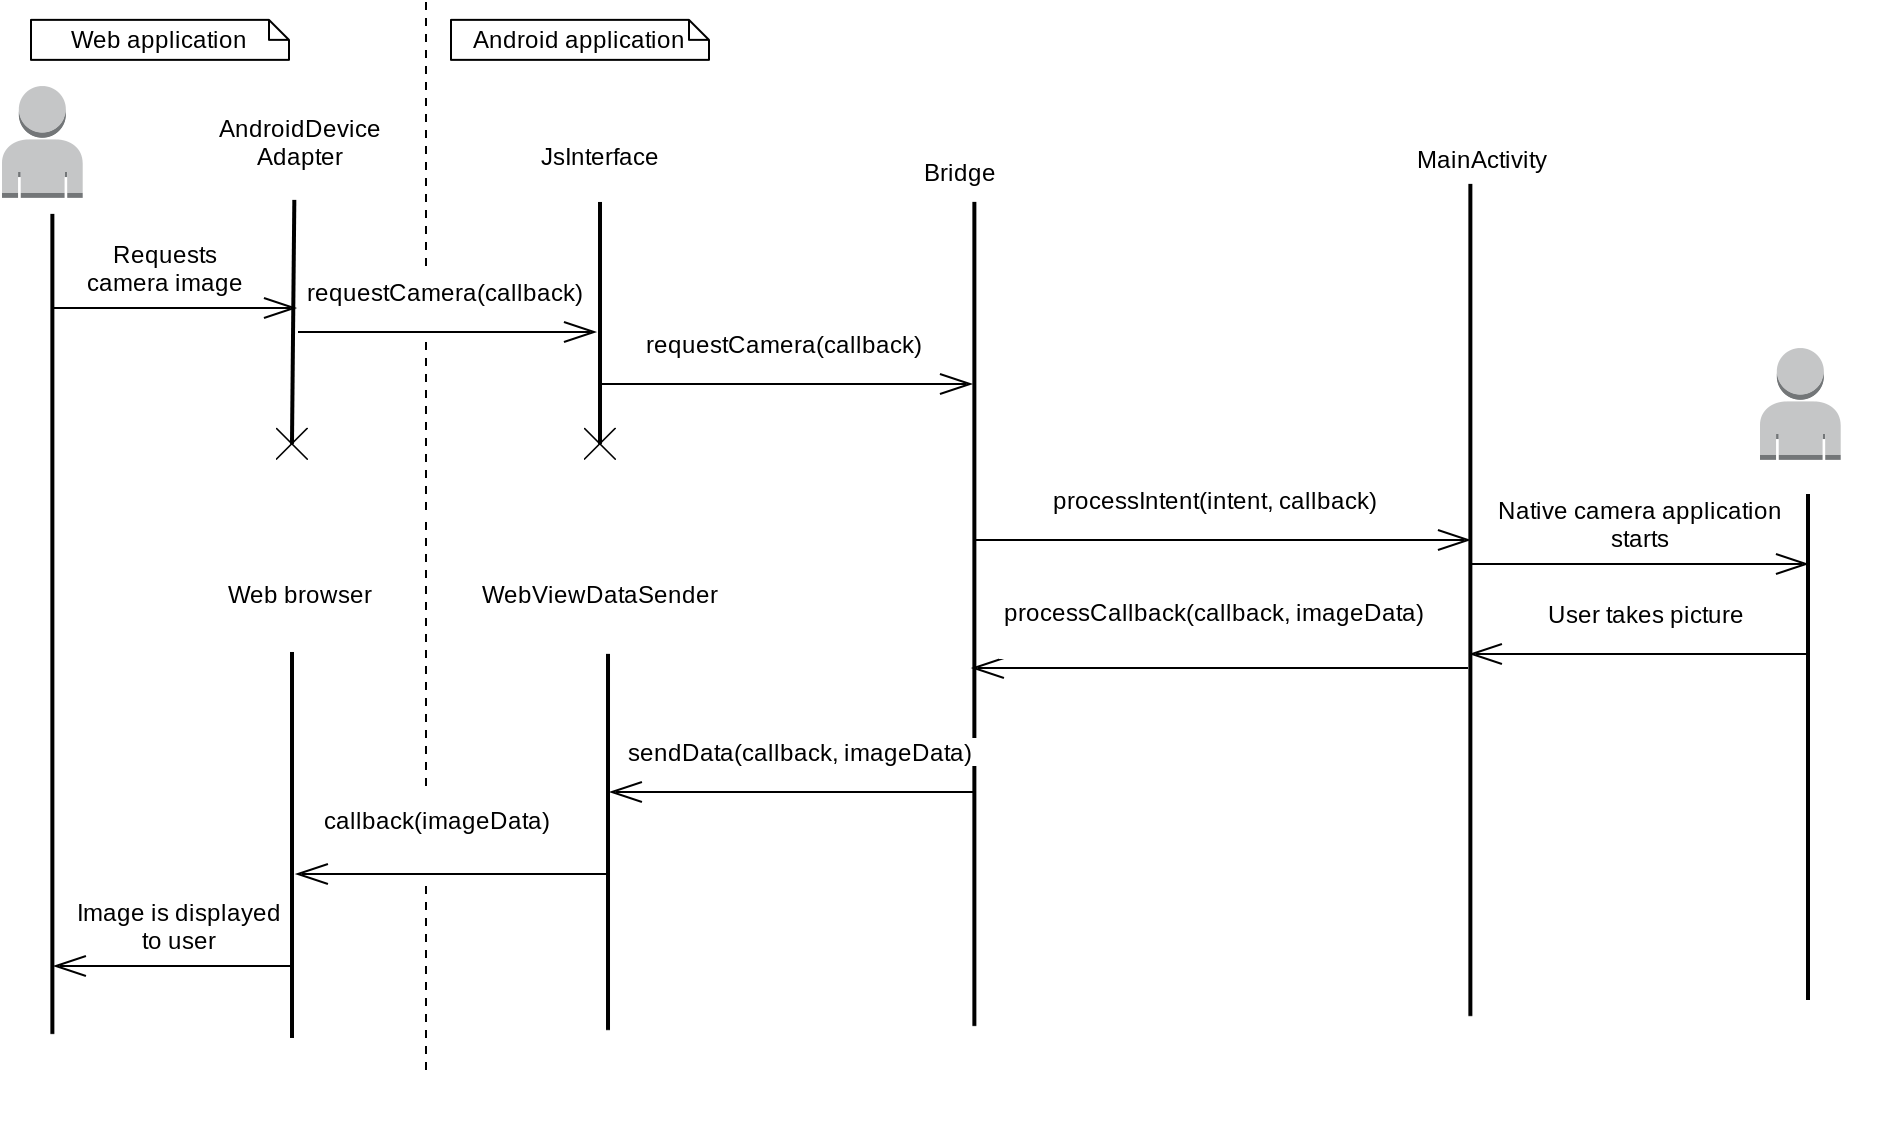
\includegraphics[width=150mm,natwidth=1000,natheight=750]{./img/androidfunctionflow.png}
    \caption{Function flowchart, single call from web application \label{fig:nativeflow}}
\end{figure}
\begin{enumerate}
	\item User action invokes a request for an image from the mobile camera.
	\item Current device adapter (see figure \ref{fig:webuml}) calls requestCamera on JsInterface, with the function name of the preferred callback function as argument.
	\item JsInterface forwards the function call to Bridge.
	\item Bridge creates the corresponding Intent and Callback, and calls processIntent on MainActivity with Intent and Callback as arguments.
	\item MainActivity gets a unique id from UniqueInteger, stores the callback in a hashmap with the id as key, and starts the intent with the id as requestcode (camera application starts).
	\item When user finishes taking a picture, the result is sent to MainActivity through onActivityResult.
	\item MainActivity finds the Callback with the same id as the processed Intent, and forwards the callback and resulting image data to Bridge through processCallback.
	\item Bridge executes the callback which in turn calls sendData on WebViewDataSender, with the image data and callback name as arguments.
	\item WebViewDataSender executes the JavaScript callback function in the WebView.
	\item The captured image is displayed to the user in the WebView.
\end{enumerate}

\section{PhoneGap}\label{sec:phonegap}
The mobile application developed in the PhoneGap framework can be found on Github at \url{https://github.com/buren-trialbee/pollux}. An overview of the application structure and functionality follows in section~\ref{subsec:application-structure-phonegap}. After this, in section~\ref{subsec:function-flow-phonegap}, a practical example is used to describe the flow of function calls when a native function is requested by the web application layer.

\subsection{Mobile application structure} \label{subsec:application-structure-phonegap}
The Android application developed using PhoneGap is a hybrid application~\ref{sec:terminology}, and is thus run within a WebView on Android. The user interface of the developed application is a HTML document containing a single inline frame~\ref{subsec:inline-frame}, which is used to load the web application front-end. To be able to embed the web application front-end the X-Frame-Options response header were removed. The logic developed for the Android application is written in JavaScript, which is loaded in the WebView. A UML-diagram representing the logic of the Android application can be seen in figure~\ref{fig:phonegapuml}, with the classes summarized below.
\begin{figure}[h!]
	\centering
    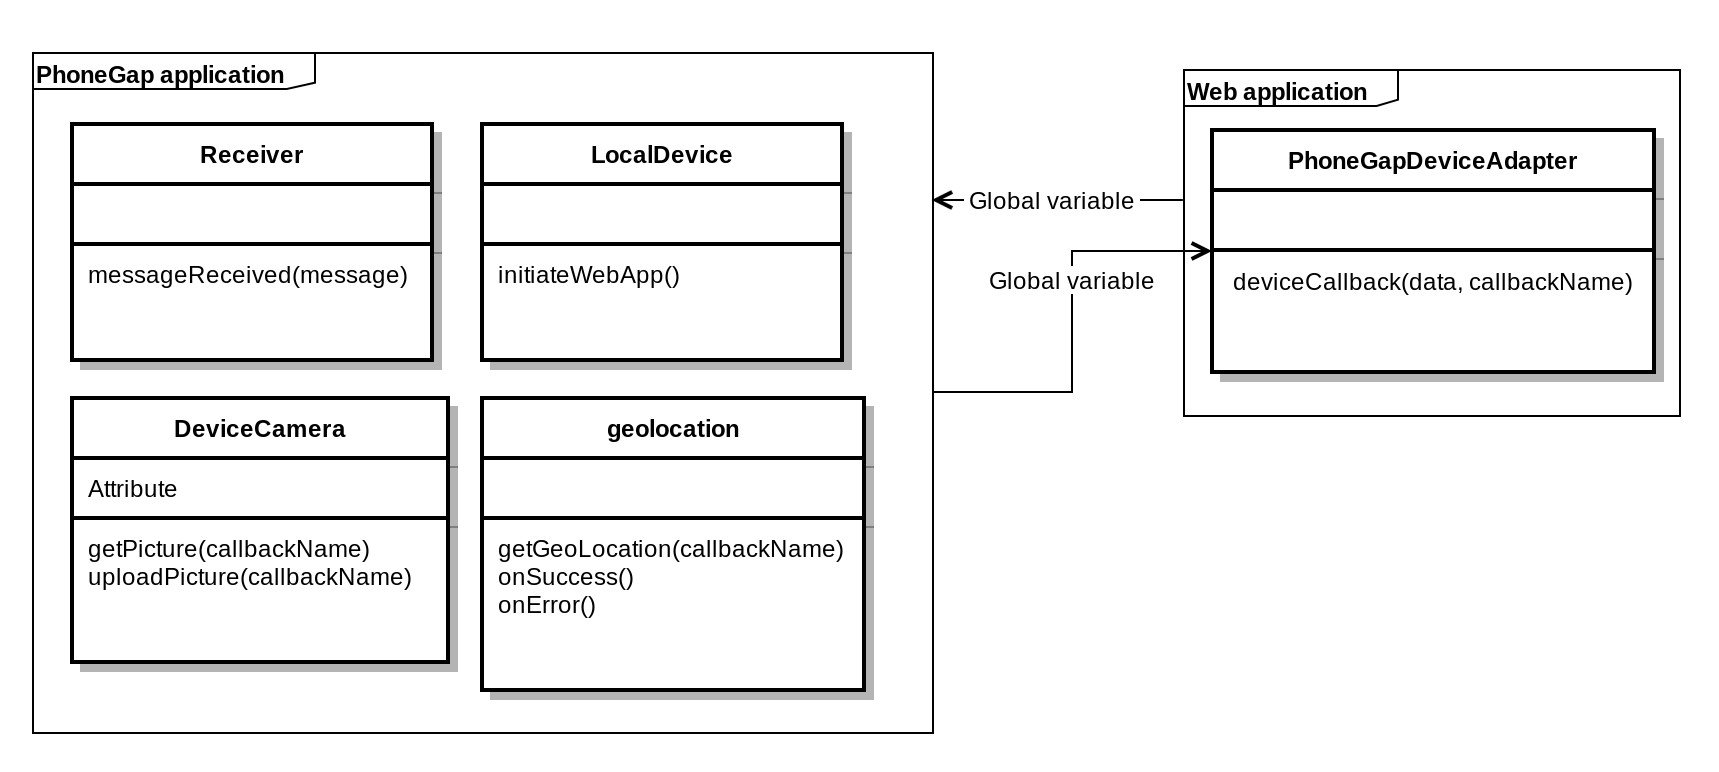
\includegraphics[width=150mm,natwidth=1000,natheight=750]{./img/phonegapuml.png}
    \caption{Structure of the phonegap application}
    \label{fig:phonegapuml}
\end{figure}

\subsubsection{Receiver}
Receiver listens to messages posted by the web application layer. A message contains a request for data from a native feature.
\label{fig:phonegapflow}
\subsubsection{LocalDevice}
LocalDevice contains a single method initiateWebApp, which is used to load the web application in an inline frame and initialize device, see figure~\ref{fig:webuml}, in the web application to the correct adapter.

\subsubsection{DeviceCamera}
DeviceCamera contains logic for invoking and receiving results from the device camera. Communication with the device camera is handled by functions provided by the PhoneGap framework. Its functions are called by Receiver upon requests from the web application layer.

\subsubsection{geolocation}
Geolocation contains logic for accessing the mobile's geolocation (GPS-position). Its functions are called by Receiver upon requests from the web application.

\subsection{Function flow}\label{subsec:function-flow-phonegap}
A more detailed view of the program flow when the web application requests an image can be seen in figure~\ref{fig:phonegapflow}, further explained below.
\begin{figure}[h!]
	\centering
    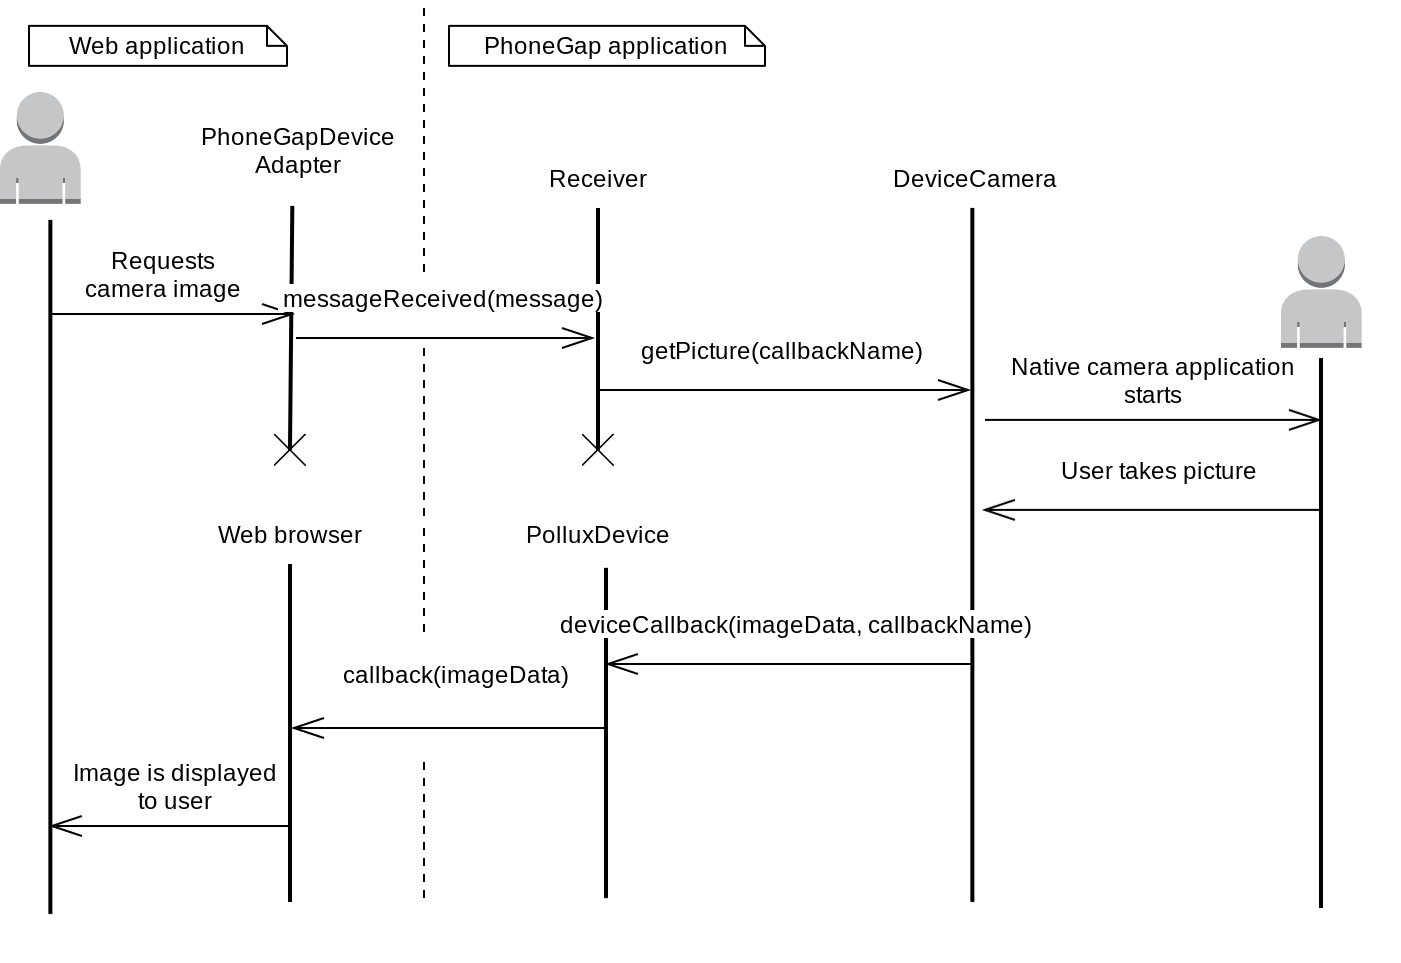
\includegraphics[width=120mm,natwidth=800,natheight=600]{./img/phonegapfunctionflow.png}
    \caption{Function flowchart, single call in web application \label{fig:phonegapflow}}
\end{figure}
\begin{enumerate}
	\item User action invokes a request for an image from the mobile camera. 
	\item Current device adapter (PhoneGapDeviceAdapter) forwards the request to the mobile application using postMessage.
	\item The message gets processed by the PhoneGap receiver which forwards the call to DeviceCamera via the getPicture function.
	\item DeviceCamera starts the camera application.
	\item When user is finished taking a picture, the result is returned to DeviceCamera.
	\item DeviceCamera returns the result to the inline frame by invoking DeviceCallback on the exposed JavaScript object, in the mobile application known as PolluxDevice.
	\item DeviceCallback calls the JavaScript callback function specified in its argument.
	\item The captured image is displayed to the user in the WebView.
\end{enumerate}


\section{Development effort}\label{sec:development-effort}
The development effort was measured using lines of code as described in section~\ref{sec:measuring-lines-of-code}. A summary of the results can be seen in the table below.

\begin{tabular}{ | l | c | r | }
    \hline
    \multicolumn{3}{|c|}{Lines of code - mobile application} \\
    \hline
	Metric & PhoneGap application &  Web application \\
	\hline
	Files & 10 & 3\\
	LLoC & 200 & 86\\	
	\hline
	\multicolumn{3}{c}{\emph{Result of code evaluation using ProjectCodeMeter}}
\end{tabular}

\begin{tabular}{ | l | c | r | }
    \hline
    \multicolumn{3}{|c|}{Lines of code - web application} \\
    \hline
	Metric & Using Android SDK & Using PhoneGap \\
	\hline
	Files & 2 & 2 \\
	LLoC & 173 & 175 \\	
	\hline
	\multicolumn{3}{c}{\emph{Result of code evaluation using ProjectCodeMeter}}
\end{tabular}

